\chapter{Testy aplikacji backendowej}

\section{Testy jednostkowe}
Testowanie aplikacji backendowej jest kluczowym elementem zapewniającym jakość i stabilność oprogramowania. W tym rozdziale przedstawiono strukturę testów jednostkowych zaimplementowanych w projecie z wykorzystaniem frameworków Spring Boot oraz JUnit 5. Testy podzielono na różne moduły, takie jak blockchain, kryptowaluty, NFT, oraz zasoby. Pozwoliło to na łatwiejsze zarządzanie i rozwój aplikacji. Testy integracyjne i wydajnościowe zostaną przeprowadzone w przyszłości.

\subsection{Testy w module Blockchain}

Moduł blockchain zawiera testy związane z obsługą różnych łańcuchów bloków, takich jak Bitcoin, Ethereum i Solana. Poniżej przedstawiano przykłady testów dla różnych podkategorii.

\subsubsection{Testy dla Bitcoin}

Przykładowy test dla klasy \texttt{BitcoinAccountControllerTest}

\begin{lstlisting}[language=Java, style=JavaStyle]
package org.example.backend.blockchain.bitcoin.accounts.controller;
import ...

class BitcoinAccountControllerTest {
    @Mock
    private BitcoinAccountService bitcoinAccountService;

    @InjectMocks
    private BitcoinAccountController bitcoinAccountController;

    @BeforeEach
    void setUp() {
        MockitoAnnotations.openMocks(this);
    }

    @Test
    void testGetAccountData_Found() {
        String address = "...";
        BitcoinAccountDto bitcoinAccountDto = new BitcoinAccountDto();
        when(bitcoinAccountService.getAllAccountData(address)).thenReturn(bitcoinAccountDto);
        ResponseEntity<BitcoinAccountDto> response = bitcoinAccountController.getAccountData(address);
        assertEquals(ResponseEntity.ok(bitcoinAccountDto), response);
        verify(bitcoinAccountService, times(1)).getAllAccountData(address);
    }

    @Test
    void testGetAccountData_NotFound() {
        String address = "testAddress";
        when(bitcoinAccountService.getAllAccountData(address)).thenReturn(null);
        ResponseEntity<BitcoinAccountDto> response = bitcoinAccountController.getAccountData(address);
        assertEquals(ResponseEntity.notFound().build(), response);
        verify(bitcoinAccountService, times(1)).getAllAccountData(address);
    }
}
\end{lstlisting}

\subsubsection{Testy dla Ethereum}
Przykładowy test dla klasy \texttt{EthereumBlockMapperTest}

\begin{lstlisting}[language=Java, style=JavaStyle]
package org.example.backend.blockchain.ethereum.block.mapper;
import ...

public class EthereumBlockMapperTest {

    @Test
    public void testMapToEthereumBlockDto() {
        EthereumBlock ethereumBlock = new EthereumBlock();
        ethereumBlock.setNumber("12345L");
        ethereumBlock.setHash("0xabc123");
        ethereumBlock.setMiner("0xminer123");

        Withdrawal withdrawal = new Withdrawal();
        withdrawal.setIndex("1");
        withdrawal.setValidatorIndex("100");
        withdrawal.setAddress("0xwithdrawalAddress");
        withdrawal.setAmount("50");

        List<Withdrawal> withdrawals = Arrays.asList(withdrawal);
        ethereumBlock.setWithdrawals(withdrawals);

        EthereumBlockDto ethereumBlockDto = EthereumBlockMapper.toDto(ethereumBlock);

        assertEquals(ethereumBlock.getNumber(), ethereumBlockDto.getNumber());
        assertEquals(ethereumBlock.getHash(), ethereumBlockDto.getHash());
        assertEquals(ethereumBlock.getMiner(), ethereumBlockDto.getMiner());
        assertEquals(ethereumBlock.getWithdrawals().size(), ethereumBlockDto.getWithdrawals().size());
        assertEquals(ethereumBlock.getWithdrawals().get(0).getIndex(), ethereumBlockDto.getWithdrawals().get(0).getIndex());
    }

    ...
}
\end{lstlisting}

\subsubsection{Testy dla Solana}

Przykładowy test dla klasy \texttt{SolanaTransactionService}

\begin{lstlisting}[language=Java, style=JavaStyle]
import .

public class SolanaTransactionServiceTest {

    @Mock
    private RestTemplate restTemplate;

    @InjectMocks
    private SolanaTransactionService solanaTransactionService;

    @BeforeEach
    public void setUp() {
        MockitoAnnotations.openMocks(this);
    }

    @Test
    public void testGetTransaction_Success() {
        String mockTransactionResponse = "{\"result\": {\"transaction\": {\"signature\": \"...\"}}}";

        when(restTemplate.postForObject(anyString(), any(), eq(String.class)))
                .thenReturn(mockTransactionResponse);

        SolanaTransactionDto expectedDto = new SolanaTransactionDto("abcd1234");

        Optional<SolanaTransactionDto> result = solanaTransactionService.getTransaction("...");

        assertTrue(result.isPresent());
        assertEquals(expectedDto.getSignature(), result.get().getSignature());
    }

    ...
}
\end{lstlisting}

Pozostałe klasy przetestowano podobnie. Łącznie wykonano 160 testów jednostkowych. % (patrz rysunek~\ref{fig:Testy}). 
Pozwoliły one na:
\begin{itemize}
    \item znalezienie i usunięcie 12 krytycznych błędów w kodzie,
    \item weryfikację poprawności działania kluczowych funkcji w izolacji,
    \item przygotowanie aplikacji na przyszłą integrację z bardziej złożonymi scenariuszami testowymi.
\end{itemize}
%%\begin{figure}[htb] % ten rysunek nic specjalnego nie wnosi, poza tym raportuje 159 testów, a nie 160
    %%\centering
    %%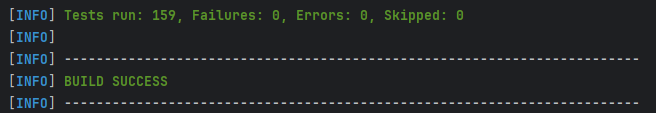
\includegraphics[width=0.8\linewidth]{./obrazy/tests.png}
    %%\caption{Testy}
    %%\label{fig:Testy}
%%\end{figure}

\section{Testy integracyjne}
Testy integracyjne planowane w przyszłości obejmą:
\begin{itemize}
    \item Weryfikację poprawności współpracy między modułami backendowymi.
    \item Sprawdzenie integracji z zewnętrznymi API, takimi jak Alchemy dla Ethereum i Solany.
    \item Testowanie interakcji z bazą danych, w tym poprawności zapisywania i odczytywania danych blockchainowych.
\end{itemize}
